%%%%%%%%%%%%%%%%%%%%%%%%%%%%%%%%%%%%%%%%%%%%%%%%%%%%%%%%%%%%%%%%%%%%%%%%%%%%%%%%
%%%%%%%%%%%%%%%%%%   Vorlage für eine Abschlussarbeit   %%%%%%%%%%%%%%%%%%%%%%%%
%%%%%%%%%%%%%%%%%%%%%%%%%%%%%%%%%%%%%%%%%%%%%%%%%%%%%%%%%%%%%%%%%%%%%%%%%%%%%%%%

% Erstellt von Maximilian Nöthe, <maximilian.noethe@tu-dortmund.de>
% ausgelegt für lualatex und Biblatex mit biber

% Kompilieren mit
% latexmk --lualatex --output-directory=build thesis.tex
% oder einfach mit:
% make

\documentclass[
  %tucolor,       % remove for less green,
  BCOR=12mm,     % 12mm binding corrections, adjust to fit your binding
  parskip=half,  % new paragraphs start with half line vertical space
  open=any,      % chapters start on both odd and even pages
  cleardoublepage=plain,  % no header/footer on blank pages
]{tudothesis}


% Warning, if another latex run is needed
\usepackage[aux]{rerunfilecheck}

% just list chapters and sections in the toc, not subsections or smaller
\setcounter{tocdepth}{1}

%------------------------------------------------------------------------------
%------------------------------ Fonts, Unicode, Language ----------------------
%------------------------------------------------------------------------------
\usepackage{fontspec}
\defaultfontfeatures{Ligatures=TeX}  % -- becomes en-dash etc.

% german language
\usepackage{polyglossia}
\setdefaultlanguage{english}

% for english abstract and english titles in the toc
\setotherlanguages{german}

% intelligent quotation marks, language and nesting sensitive
\usepackage[autostyle]{csquotes}

% microtypographical features, makes the text look nicer on the small scale
\usepackage{microtype}

%------------------------------------------------------------------------------
%------------------------ Math Packages and settings --------------------------
%------------------------------------------------------------------------------

\usepackage{amsmath}
\usepackage{amssymb}
\usepackage{mathtools}

% Enable Unicode-Math and follow the ISO-Standards for typesetting math
\usepackage[
  math-style=ISO,
  bold-style=ISO,
  sans-style=italic,
  nabla=upright,
  partial=upright,
]{unicode-math}
\setmathfont{Latin Modern Math}

% nice, small fracs for the text with \sfrac{}{}
\usepackage{xfrac}


%------------------------------------------------------------------------------
%---------------------------- Numbers and Units -------------------------------
%------------------------------------------------------------------------------

\usepackage[
  separate-uncertainty=true,
  per-mode=symbol-or-fraction,
]{siunitx}
\sisetup{math-micro=\text{µ},text-micro=µ}

%------------------------------------------------------------------------------
%-------------------------------- tables  -------------------------------------
%------------------------------------------------------------------------------

\usepackage{booktabs}       % \toprule, \midrule, \bottomrule, etc

%------------------------------------------------------------------------------
%-------------------------------- graphics -------------------------------------
%------------------------------------------------------------------------------

\usepackage{graphicx}
\usepackage{grffile}
% allow figures to be placed in the running text by default:
\usepackage{scrhack}
\usepackage{float}
\floatplacement{figure}{htbp}
\floatplacement{table}{htbp}

% keep figures and tables in the section
\usepackage[section, below]{placeins}


%------------------------------------------------------------------------------
%---------------------- customize list environments ---------------------------
%------------------------------------------------------------------------------

\usepackage{enumitem}

%------------------------------------------------------------------------------
%------------------------------ Bibliographie ---------------------------------
%------------------------------------------------------------------------------

\usepackage[
  backend=biber,   % use modern biber backend
  autolang=hyphen, % load hyphenation rules for if language of bibentry is not
                   % german, has to be loaded with \setotherlanguages
                   % in the references.bib use langid={en} for english sources
  sorting=none,
]{biblatex}
\addbibresource{references.bib}  % the bib file to use

\DefineBibliographyStrings{english}{andothers = {{et\,al\adddot}}}  % replace u.a. with et al.
\usepackage{bibstyle}
\usepackage{emptypage}
% Last packages, do not change order or insert new packages after these ones
\usepackage[pdfusetitle, unicode, linkbordercolor=tugreen]{hyperref}
\usepackage{bookmark}
\usepackage[shortcuts]{extdash}
%\usepackage{graphicx,subfigure}
%------------------------------------------------------------------------------
%-------------------------    Angaben zur Arbeit   ----------------------------
%------------------------------------------------------------------------------

\author{Christopher Krause}
\title{Track reconstruction for low energy protons using Corryvreckan}
\date{2021}
\birthplace{Mainz}
\chair{Lehrstuhl für Experimentelle Physik IV}
\division{Fakultät Physik}
%\thesisclass{Bachelor of Science}
%\submissiondate{12. Juli 2019}
%\firstcorrector{Dr.~Jens Weingarten}
%\secondcorrector{Prof.~Dr.~Dr.~Wolfgang Rhode}

% tu logo on top of the titlepage
\titlehead{\includegraphics[height=1.5cm]{logos/tu-logo.pdf}}

\begin{document}
\frontmatter
%\thispagestyle{empty}
\setcounter{page}{2}
\section*{Hinweise}
Empfohlen wird die Verwendung dieser Vorlage mit der jeweils aktuellsten TeXLive Version (Linux, Windows) bzw. MacTeX Version (MacOS).
Aktuell ist dies TeXLive 2016. Download hier:
\begin{center}
  \ttfamily\url{https://www.tug.org/texlive/}
\end{center}
Bei Verwendung von TexLive Versionen 2014 und älter sollte
die Zeile
\begin{center}
\verb+\RequirePackage{fixltx2e}+ 
\end{center}
als erste Zeile der Präambel noch vor der Dokumentenklasse eingefügt werden.
Dies lädt diverse Bugfixes für LaTeX, die ab TexLive 2015 Standard sind.

Die Vorlage \texttt{thesis.tex} ist für die Kompilierung mit \texttt{lualatex} ausgelegt, mit wenigen Anpassungen kann sie aber auch mit \texttt{pdflatex} oder \texttt{xelatex} verwendet werden. 
Die Dokumentenklasse \texttt{tudothesis.cls} kann mit allen drei Programmen verwednet werden.

Achten Sie auch auf die Kodierung der Quelldateien.
Bei Verwendung von Xe\LaTeX\ oder Lua\LaTeX\ (empfohlen) müssen die
Quelldateien UTF-8 kodiert sein.
Bei Verwendung von pdf\LaTeX\ nutzen Sie die Pakete \texttt{inputenc} und \texttt{fontenc} mit der korrekten Wahl der Kodierungen.

Eine aktuelle Version dieser Vorlage steht unter 
\begin{center}
  \ttfamily\url{https://github.com/maxnoe/tudothesis}
\end{center}
zur Verfügung.

Alle verwendeten Pakete werden im \LaTeX{} Kurs von Pep et al.\ erklärt:
\begin{center}
  \ttfamily\url{http://toolbox.pep-dortmund.org/notes}
\end{center}

Für Rückmeldungen und bei Problemen mit der Klasse oder Vorlage, bitte ein \emph{Issue} auf GitHub aufmachen oder eine Email an
\href{mailto:maximilian.noethe@tu-dortmund.de}{maximilian.noethe@tu-dortmund.de} schreiben.

Wenn Sie die Dokumentenklasse mit der Option \texttt{tucolor} laden, werden verschiedene Elemente in TU-Grün gesetzt.

\maketitle

% Gutachterseite
\makecorrectorpage

% hier beginnt der Vorspann, nummeriert in römischen Zahlen
\thispagestyle{plain}

\section*{Kurzfassung}
Die Protonentherapie ist, wegen ihrer höheren Präzision der Energiedeposition, eine wirkungsvolle Alternative zu herkömmlichen Röntgentherapie.
Auftretende Unsicherheiten durch die Verwendung von Röntgen Computertomographie können mit dem Verfahren der Protonen Computertomographie reduziert werden.
Um damit einen Bestrahlungsplan anfertigen zu können ist es nötig die Spuren der Protonen durch den Körper mithile von Detektoren zu rekonstruieren. \\
In dieser Arbeit wird die neue Spurrekonstruktions Software Corryvreckan mit der in Zukunft eingestellten Software EUTelescope auf ihre Funktionalität im
Rekonstruieren von Spuren in Testbeam Experimenten untersucht. Es wird gezeigt, dass Corryvreckan in der Lage ist Spuren mit vergleichbarer Qualität zu rekonstruieren.\\
Des Weiteren werden Simulation von Protonstrahlen durch ein Teleskop erstellt, um die rekonstruierbarkeit von niederenergetischen Protonen
mit Corryvreckan zu analysieren. (Hier noch Erbenis)

\section*{Abstract}
\begin{english}




\end{english}

\tableofcontents

\mainmatter
% Hier beginnt der Inhalt mit Seite 1 in arabischen Ziffern
\chapter{Introduction}
The investigation of particles and their properties is the foundation of particle physics. With the development of the standard model in the past century, particles
and their interactions with other particles could be better understood. The fundamental particles can be divided into quarks and leptons, making up the matter in the universe,
gauge bosons, which mediate three of the fundamental forces, and the Higgs boson.

In order to analyse interactions of particles, they are accelerated and brought to collision inside of particle colliders. The particles created in such collisions
can be detected with a surrounding detector system and thus the events can be reconstructed, giving an insight into their properties. It is, therefore, crucial to have
an optimal working detector to analyse the produced data precisely.
Currently, the largest collider is
the Large Hadron Collider (LHC) \cite{lhc} located at CERN, which is able to accelerate protons up to
a centre of mass energy of $\SI{14}{\tera\eV}$.
It operates since 2008 and helped particle physicists in finding the last missing particle of the standard model, the Higgs boson \cite{higgs}\cite{higgs_cms}, as well as giving more insight
into properties of particles like the top quark. Standard model parameters can be measured with greater precision, which improves the understanding of fundamental physical processes
and enables physicists to test their theories. %Physics beyond the standard model is also searched for at the LHC with great interest.

Besides the use of detectors in high-energy physics experiments, they are also a crucial part of medical equipment, specifically used for radiative treatments. \\
The idea to use protons as an effective particle for the treatment of cancer arose in 1946 \cite{1946} and over the years it proved to have several advantages over
conventional x-ray radiation therapy. To apply proton therapy, a radiation plan has to be created to determine the location of the tumor and the dose of the radiation.
For that purpose tomography scans create images of the inside of patients, enabling the precise irradiation of tumors.
The benefits of using protons for tomography scans in comparison to x-ray tomography scans for proton therapy caused a growing interest in this technique \cite{pbt}. \\
In order to create images with proton computed tomography, the reconstruction of proton tracks traversing the human body and the measurement of their energy is necessary.

This thesis focuses on the reconstruction of proton tracks under conditions present in proton computed tomography scans. To achieve that, the new track reconstruction software
Corryvreckan \cite{corryvreckan} is analysed based on its capability of reconstructing tracks in comparison to the EUTelescope framework \cite{gbl} known
for its long use in detector physics. Furthermore,
it is used to reconstruct
proton tracks, which are generated in Allpix$^2$ \cite{allpix} simulations to investigate the possibility of making proton computed tomography scans feasible with this framework.


%An interest for the imaging
%technique of proton computed tomogrophy came up around 1990, with proton therapy gaining in popularity due to its advantages over conventional x-ray therapy.
%In order to create images with proton computed tomography, the reconstruction of proton tracks traversing the human body is


%The ATLAS detector is one of the four large experiments at the LHC. % and the largest particle detector with a length of $\SI{46}{\meter}$ and a diameter of $\SI{25}{\meter}$.
%It was build to observe many different type of physical phenomena including the detection of the higgs boson in 2012 along with the CMS experiment. In order
%to identify the produced particles in the collisions, many layers of different detectors make up the entire ATLAS detector. The most inner layer is the pixel detector, which
%is composed of pixel sensor modules to detect particles and reconstruct their tracks.
%
%To measure the efficiency of pixel sensors,
%particle tracks are reconstructed in testbeam facilities with a telescope setup made of Mimosa26 pixel sensors to investigate the devices under test (DUT), which are
%placed inside the telescope. These measurements are necessary to ensure an optimal performance of sensor modules inside the experiments.

\chapter{The Large Hadron Collider}
%\section{Siliziumdetektoren}
The LHC was build between 1998 and 2008 by the European Organization for Nuclear Research (CERN) in collaboration with 10000 scientist from over 100 countries
and lies in a $\SI{27}{\kilo\meter}$ tunnel 175 metres underground in Switzerland near Geneva. It is a proton-proton synchrotron, which uses
the systems to accelerate the protons before they are injected into the main accelerator. The linear particle accelerator LINAC 4 generates $\SI{160}{\mega\eV}$
negative hydrogen ions and launches them into the Proton Synchrotron Booster (PSB). Here, the electrons are removed from the hydrogen ions, leaving only the nucleus
consisting of one proton, which then enters the Super Proton Synchrotron (SPS). It increases the protons energy to $\SI{450}{\GeV}$ and feeds them to the
LHC, where to opposing proton beams are accelerated. In the main ring,
the protons are accumulated to bunches and accelerated to their maximum energy of $\SI{13}{\tera\eV}$ in 20 minutes.

At four locations, the two proton beams
are crossed, making it possible for them to collide. Around these interaction points, the four large experiments, ATLAS, CMS, LHCb and Alice are operated.
Occasionaly lead nuclei are accelerated to study matter under extreme conditions at the ALICE experiment. The ATLAS and CMS experiment are general-purpose detectors for
high energy physics. They differ on their technical design to achieve their goal and enable to corrobate each others results.
LHCb is an asymmetric particle detector specialized in measuring the parameters of CP violation in B-meson decays.
Further experiments at the LHC include TOTem, LHCf, MoEDAL and FASER, which focus on specialized research. Figure \ref{fig:lhc_aufbau} shows the schematic depiction
of the LHC.

\begin{figure}[H]
  \centering
  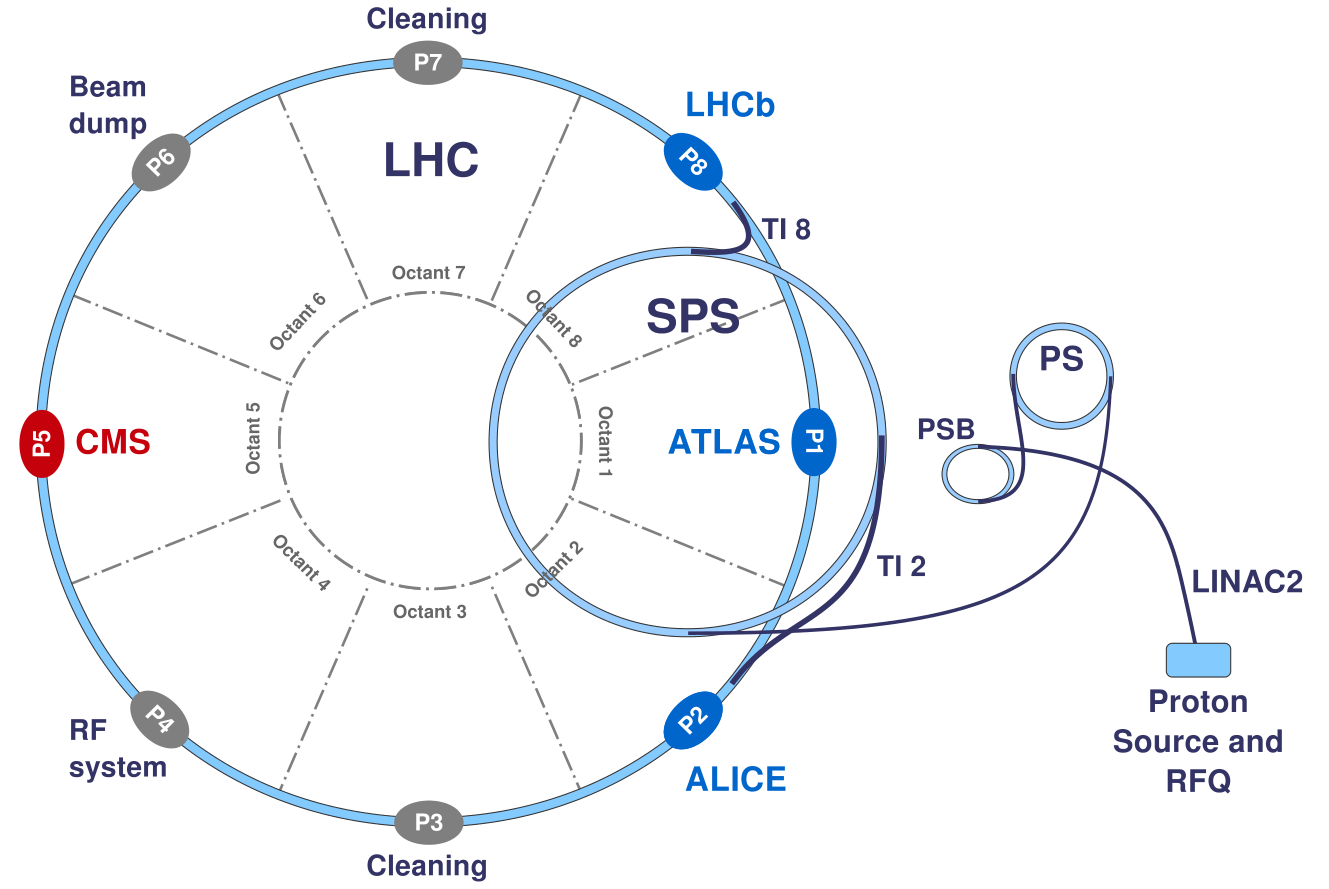
\includegraphics[height=0.4\textwidth]{images/lhc_aufbau.png}
  \caption{Schematic representation of the CERN accelerator complex (not to scale)\cite{lhc_aufbau}.}
  \label{fig:lhc_aufbau}
\end{figure}

After the second run from 2015 to 2018 followed the Long Shutdown 2 (LS2) until 2021 in order to upgrade the accelerator. The goal is to increase the luminosity by a factor of 10 by
implementing High Luminosity Large Hadron Collider (HL-LHC) in the Long Shutdown 3 (LS3), which is planned to be operational in 2026. Figure \ref{fig:lhc_plan} shows the timeline
of LHC programme.

\begin{figure}
  \centering
  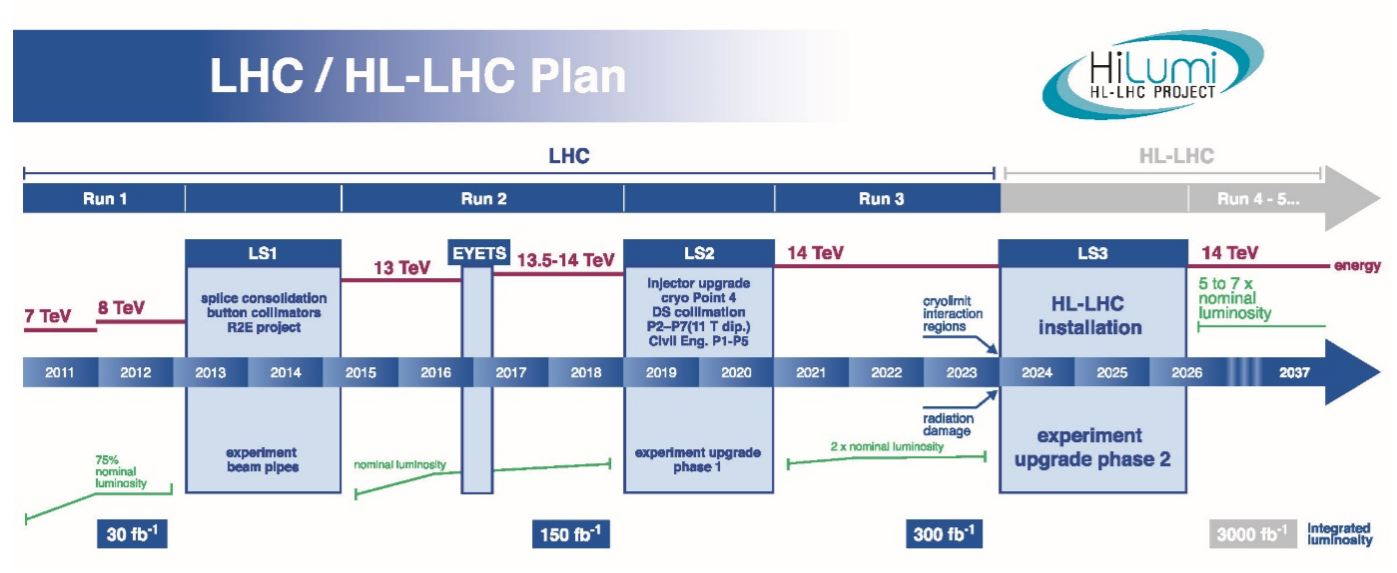
\includegraphics[height=0.4\textwidth]{images/lhc_plan.png}
  \caption{Timeline of the operational phases and Shutdowns of the LHC. The energy of accelerated protons in each phase is shown in red and the luminosity in green \cite{lhc_plan}.}
  \label{fig:lhc_plan}
\end{figure}

\chapter{Comparison of EUTelescope and Corryvreckan}\label{make}

\chapter{Zusammenfassung}


%\appendix
% Hier beginnt der Anhang, nummeriert in lateinischen Buchstaben
\chapter{Appendix}
%\section{Bin entries of cluster size plots}
  \begin{table}
    \centering
    \begin{tabular}{c | c c}
      \toprule
      Bin & Corryvreckan & EUTelescope \\
      \midrule
      1      & 3934209 & 3934209            \\
      2      & 1136782 & 1136782           \\
      3      & 295505  & 295505           \\
      4      & 288595  & 288595           \\
      5      & 50477   & 50477           \\
      6      & 42916   & 42916           \\
      7      & 31800   & 31800           \\
      8      & 23759   & 23759           \\
      9      & 15892   & 15892           \\
      10     & 11378   & 11378           \\
      11     & 8030    & 8030           \\
      12     & 7472    & 7472           \\
      13     & 5576    & 5576           \\
      14     & 4332    & 4332           \\
      15     & 3155    & 3155           \\
      16     & 3740    & 3740           \\
      17     & 2744    & 2744           \\
      18     & 1917    & 1917           \\
      19     & 1357    & 1357           \\
      20     & 1022    & 1022           \\
      21-30  & 990434  & 990434            \\
      31-40  & 634     & 634       \\
      41-50  & 986247  & 986247        \\
      51-59  & 207     & 207            \\
    \end{tabular}
    \caption{Bin entries of the cluster size plots of Corryvreckan and EUTelescope for the first plane shown in figure \ref{fig:cluster_size}.}
    \label{tab:cluster_sizes}
  \end{table}

\clearpage

\begin{lstlisting}[caption={Configuration file of Corryvreckan for the testbeam anaylsis of June 2020 Batch 3}]
[Corryvreckan]
detectors_file = output/updated_real_geometry.conf
detectors_file_updated = output/updated_real_geometry.conf
histogram_file=histogram_testbeam_realdata.root

[EventLoaderEUDAQ]
file_name = "/path_to_data.raw"
long_detector_id = false

[Clustering4D]

[Correlations]

[Prealignment]
method= gauss_fit

[Tracking4D]
track_model = "gbl"
exclude_dut = true
spatial_cut_abs = 120um, 120um
timing_cut_abs = 350ns
min_hits_on_track = 6
momentum = 5GeV

[AlignmentTrackChi2]
iterations = 3

[DUTAssociation]
spatial_cut_abs =500um, 200um
time_cut_abs = 230us

[AlignmentDUTResidual]
iterations = 3

[AnalysisDUT]
chi2ndof_cut = 5
\end{lstlisting}

\clearpage
\begin{lstlisting}[caption={Detector file of Corryvreckan for the testbeam anaylsis of June 2020 Batch 3}]
[plane0]
material_budget = 0.00075
number_of_pixels = 1152, 576
orientation = -0.659875deg,5.4639deg,0.350077deg
orientation_mode = "xyz"
pixel_pitch = 18.4um,18.4um
position = -658.122um,-147.97um,0
spatial_resolution = 5.4um,5.4um
time_resolution = 230us
type = "mimosa26"

[plane1]
material_budget = 0.00075
number_of_pixels = 1152, 576
orientation = -0.47332deg,4.61982deg,-0.117972deg
orientation_mode = "xyz"
pixel_pitch = 18.4um,18.4um
position = -587.717um,-133.671um,111mm
spatial_resolution = 5.4um,5.4um
time_resolution = 230us
type = "mimosa26"

[plane2]
material_budget = 0.00075
number_of_pixels = 1152, 576
orientation = -0.136822deg,3.69758deg,0.117857deg
orientation_mode = "xyz"
pixel_pitch = 18.4um,18.4um
position = -386.259um,-237.934um,222mm
spatial_resolution = 5.4um,5.4um
time_resolution = 230us
type = "mimosa26"

[plane110]
material_budget = 0.003
number_of_pixels = 401, 193
orientation = 8.55701deg,46.4751deg,3.61319deg
orientation_mode = "xyz"
pixel_pitch = 50um,50um
position = -6.65508mm,-83.16um,355mm
roi = [[266,1],[266,193],[401,1],[401,193]]
role = "dut"
spatial_resolution = 14um,14um
time_resolution = 200ns
type = "rd53a"

[plane112]
material_budget = 0.003
number_of_pixels = 401, 193
orientation = 0,-0,-0.0220589deg
orientation_mode = "xyz"
pixel_pitch = 50um,50um
position = -5.5818mm,448.868um,425mm
roi = [[266,1],[266,193],[401,1],[401,193]]
role = "dut"
spatial_resolution = 14um,14um
time_resolution = 200ns
type = "rd53a"

[plane3]
material_budget = 0.00075
number_of_pixels = 1152, 576
orientation = 0,0,0
orientation_mode = "xyz"
pixel_pitch = 18.4um,18.4um
position = 0,0,571mm
role = "reference"
spatial_resolution = 5.4um,5.4um
time_resolution = 230us
type = "mimosa26"

[plane4]
material_budget = 0.00075
number_of_pixels = 1152, 576
orientation = 1.15485deg,-0.940166deg,0.246945deg
orientation_mode = "xyz"
pixel_pitch = 18.4um,18.4um
position = -274.402um,134.999um,681mm
spatial_resolution = 5.4um,5.4um
time_resolution = 230us
type = "mimosa26"

[plane5]
material_budget = 0.00075
number_of_pixels = 1152, 576
orientation = 0.735678deg,-1.16597deg,-0.0280176deg
orientation_mode = "xyz"
pixel_pitch = 18.4um,18.4um
position = -482.401um,213.683um,793mm
spatial_resolution = 5.4um,5.4um
time_resolution = 230us
type = "mimosa26"

[plane21]
material_budget = 0.003
number_of_pixels = 80, 336
orientation = 179.875deg,3.70623deg,89.9804deg
orientation_mode = "xyz"
pixel_pitch = 250um,50um
position = -1.42585mm,504.062um,835mm
role = "dut"
spatial_resolution = 72um,14um
time_resolution = 25ns
type = "fei4"
\end{lstlisting}

\clearpage

\begin{lstlisting}[caption={Configuration file of EUTelescope for the testbeam anaylsis of June 2020 Batch 3}]
[DEFAULT]
# The path to this config file
BasePath                = /path_to_config_file

# Set the folder which contains the raw/native data files
NativePath              = /path_to_data_file

#The location of the steering templates
TemplatePath    = %(BasePath)s/steering-templates

# The GEAR file describing the detector geometry,
# this is passed from the runlist.csv
GearFile                = @GearGeoFile@

# Beam Energy is retrieved from the runlist.csv
BeamEnergy              = @BeamEnergy@

# Path to the GEAR files
GearFilePath    = %(BasePath)s/gear

# The XML file with histogram information
HistoInfoFile   = %(TemplatePath)s/histoinfo.xml

# Formats the output;
# @RunNumber@ is the current run number
# padded with leading zeros to 6 digits
FilePrefix              = run@RunNumber@

# Skip events in a run; set to 0 for all data
SkipNEvents             = 0

# Output subfolder structure
OutPath         = %(BasePath)s/output
DatabasePath    = %(OutPath)s/database
HistogramPath   = %(OutPath)s/histograms
LcioPath        = %(OutPath)s/lcio
LogPath         = %(OutPath)s/logs
TBTrackFilePath = %(OutPath)s/tbtrack

# Limit processing of a run to a certain number of events
MaxRecordNumber = 1000000000

# The verbosity used by the EUTelescope producers
Verbosity               = MESSAGE5

# After how many events you want a "Processing event XXXX" message
NEventsMessage  = 2500

[converter]
# How many events for noisy pixel analysis
NoOfEvents              = 100000

M26SensorVec            = 0 1 2 3 4 5
FiringFreqCutM26        = 0.005

APIXSensorVec           = 110 112 21
FiringFreqCutAPIX       = 0.001

[clustering]

[hitmaker]
# ID of fixed Sensor for correlation and alignemnt
FixedPlane              = 3

#Number of events used for Correlator and PreAligner
NoEvents                = 100000

#Residual cuts for Correlator and PreAligner
ResidualsXMin   = -3. -3. -3.  -10. -10.  -3. -3. -3.  -10.
ResidualsXMax   =  3.  3.  3.   10.  10.   3.  3.  3.   10.
ResidualsYMin   = -3. -3. -3.  -10. -10.  -3. -3. -3.  -10.
ResidualsYMax   =  3.  3.  3.   10.  10.   3.  3.  3.   10.


[alignGBL]
#Template for steering file is the same in all the alignment iterations
TemplateFile    = alignGBL-tmp.xml

MaxTrackCandidatesTotal = 100000

GearFile                = @GearGeoFile@@RunNumber@_pre.xml
Iteration               = 0

# Number of alignment constants used.
AlignMode               = XYZShiftsRotXYZ

UpstreamTriplet         = 0 1 2
LastUpstreamSensor      = 2
DownstreamTriplet       = 3 4 5

FixedPlanes             = 0 5
FixedZShift             = 0 1 2 110 112 3 4 5 21

# res = pitch/sqrt(12)
resMim                  = 0.0052
resRD531X               = 0.0289
resRD531Y               = 0.0072
resRD532XY              = 0.0144
resFEI4X                = 0.0722
resFEI4Y                = 0.0144

# Both DUTs are 50x50
ResolutionX = %(resMim)s %(resMim)s %(resMim)s %(resRD532XY)s
%(resRD532XY)s %(resMim)s %(resMim)s %(resMim)s %(resFEI4X)s
ResolutionY = %(resMim)s %(resMim)s %(resMim)s %(resRD532XY)s
%(resRD532XY)s %(resMim)s %(resMim)s %(resMim)s %(resFEI4Y)s

UpstreamTripletCut              = 0.2
DownstreamTripletCut            = 0.2
UpstreamSlopeCut                = 3.0
DownstreamSlopeCut              = 3.0
TripletMatchingCut              = 0.5
DUTCuts                         = 1.0 1.0

[alignGBL1]
#Template for steering file is the same in all the alignment iterations
TemplateFile    = alignGBL-tmp.xml

MaxTrackCandidatesTotal = 100000

GearFile  = @GearGeoFile@@RunNumber@_pre_alignGBL0.xml
Iteration = 1

#Number of alignment constants used.
AlignMode               = XYZShiftsRotXYZ

UpstreamTriplet         = 0 1 2
LastUpstreamSensor      = 2
DownstreamTriplet       = 3 4 5

FixedPlanes             = 0 5
FixedZShift             = 0 1 2 110 112 3 4 5 21

# res = pitch/sqrt(12)
resMim                  = 0.0052
resRD531X               = 0.0289
resRD531Y               = 0.0072
resRD532XY              = 0.0144
resFEI4X                = 0.0722
resFEI4Y                = 0.0144

# Both DUTs are 50x50
ResolutionX = %(resMim)s %(resMim)s %(resMim)s %(resRD532XY)s
%(resRD532XY)s %(resMim)s %(resMim)s %(resMim)s %(resFEI4X)s
ResolutionY = %(resMim)s %(resMim)s %(resMim)s %(resRD532XY)s
%(resRD532XY)s %(resMim)s %(resMim)s %(resMim)s %(resFEI4Y)s

UpstreamTripletCut              = 0.2
DownstreamTripletCut            = 0.2
UpstreamSlopeCut                = 3.0
DownstreamSlopeCut              = 3.0
TripletMatchingCut              = 0.5
DUTCuts                         = 1.0 1.0

[alignGBL2]
#Template for steering file is the same in all the alignment iterations
TemplateFile    = alignGBL-tmp.xml

MaxTrackCandidatesTotal = 100000

GearFile = @GearGeoFile@@RunNumber@_pre_alignGBL0_alignGBL1.xml
Iteration = 2

#Number of alignment constants used.
AlignMode               = XYZShiftsRotXYZ

UpstreamTriplet         = 0 1 2
LastUpstreamSensor      = 2
DownstreamTriplet       = 3 4 5

FixedPlanes             = 0 5
FixedZShift             = 0 1 2 110 112 3 4 5 21

# res = pitch/sqrt(12)
resMim                  = 0.0052
resRD531X               = 0.0289
resRD531Y               = 0.0072
resRD532XY              = 0.0144
resFEI4X                = 0.0722
resFEI4Y                = 0.0144

# Both DUTs are 50x50
ResolutionX  = %(resMim)s %(resMim)s %(resMim)s %(resRD532XY)s
%(resRD532XY)s %(resMim)s %(resMim)s %(resMim)s %(resFEI4X)s
ResolutionY  = %(resMim)s %(resMim)s %(resMim)s %(resRD532XY)s
%(resRD532XY)s %(resMim)s %(resMim)s %(resMim)s %(resFEI4Y)s

UpstreamTripletCut              = 0.03
DownstreamTripletCut            = 0.03
UpstreamSlopeCut                = 2.00
DownstreamSlopeCut              = 2.00
TripletMatchingCut              = 0.20
DUTCuts                         = 0.3 0.3

[fitGBL]
#Template for steering file is the same in all the alignment iterations
TemplateFile    = fitGBL-tmp.xml

GearFile = @GearGeoFile@@RunNumber@_pre_alignGBL0_alignGBL1_alignGBL2.xml

UpstreamTriplet         = 0 1 2
LastUpstreamSensor      = 2
DownstreamTriplet       = 3 4 5

#Planes which should be excluded from track fitting:
DUTPlanes               = 110 112 21

# res = pitch/sqrt(12)
resMim                  = 0.0052
resRD531X               = 0.0289
resRD531Y               = 0.0072
resRD532XY              = 0.0144
resFEI4X                = 0.0722
resFEI4Y                = 0.0144

# Both DUTs are 50x50
ResolutionX = %(resMim)s %(resMim)s %(resMim)s %(resRD532XY)s
%(resRD532XY)s %(resMim)s %(resMim)s %(resMim)s %(resFEI4X)s
ResolutionY = %(resMim)s %(resMim)s %(resMim)s %(resRD532XY)s
%(resRD532XY)s %(resMim)s %(resMim)s %(resMim)s %(resFEI4Y)s

UpstreamTripletCut              = 0.03
DownstreamTripletCut            = 0.03
UpstreamSlopeCut                = 2.00
DownstreamSlopeCut              = 2.00
TripletMatchingCut              = 0.20
DUTCuts                         = 0.3 0.3

OutputPlanes    = 110 112 21
\end{lstlisting}

\begin{lstlisting}[caption={Allpix$^2$ simulation for 50000 protons with an energy of $\SI{100}{\giga\eV}$}]
[Allpix]
log_level = "WARNING"
log_format = "DEFAULT"
detectors_file = path_to_detector_file.conf
number_of_events = 50000
random_seed_core = 0
random_seed = 0

[GeometryBuilderGeant4]
world_material = "air"
world_margin_percentage = 0

[DepositionGeant4]
physics_list = QBBC
particle_type = "proton"
source_energy = 100GeV
source_position = 0 0 -200cm
source_type = "beam"
beam_divergence = 0mrad 0mrad
beam_size = 3mm
beam_direction = 0 0 1
number_of_particles = 1
max_step_length = 1um

[ElectricFieldReader]
type= "ibl_planar"
model="linear"
bias_voltage= -100V
depletion_depth= 200um

[GenericPropagation]
type = "ibl_planar"
temperature = 293K
charge_per_step = 300

[SimpleTransfer]
type = "ibl_planar"
max_depth_distance = 250um

[DefaultDigitizer]
type = "ibl_planar"
\end{lstlisting}

\begin{lstlisting}[caption={Allpix$^2$ geometry file for all simulations}]
[telescope0]
type = "ibl_planar"
position = 0 0 -44cm
orientation = 0deg 0 0

[telescope1]
type = "ibl_planar"
position = 0 0 -37cm
orientation = 0deg 0deg 90deg

[telescope2]
type = "ibl_planar"
position = 0 0 -30cm
orientation = 0deg 0 0

[dut0]
type = "ibl_planar"
position = 0 0 10cm
orientation = 0deg 0 0

[telescope3]
type = "ibl_planar"
position = 0 0 50cm
orientation = 0deg 0 0

[telescope4]
type = "ibl_planar"
position = 0 0 57cm
orientation = 0deg 0deg 90deg

[telescope5]
type = "ibl_planar"
position = 0 0 64cm
orientation = 0deg 0 0
\end{lstlisting}


\backmatter
\printbibliography

%\cleardoublepage
%\thispagestyle{empty}
\section*{Danksagung}

An dieser Stelle möchte ich mich bei all denjenigen bedanken, die mich während
der Anfertigung meiner Masterarbeit unterstützt haben. \\
Zunächst möchte ich mich bei Dr. Jens Weingarten bedanken, der die Erstkorrektur dieser Arbeit übernommen hat und mir stets wichtige Denkanstöße
gegeben hat.\\
Weiter möchte ich mich bei Dr. Kevin Kröninger bedanken, dass er mir ermöglichte an diesem Lehrstuhl meine Masterarbeit zu schreiben. \\
Ebenso gilt mein Dank den Mitgliedern der Detektor Upgrade Abteilung die mich schon zu meinen Bachelorzeiten herzlich in ihren Reihen willkommen hieß. \\
Auch den restlichen Mitgliedern des Lehrstuhls danke ich herzlich für den regen und konstruktiven Austausch in unseren wöchentlichen Meetings.

Dr. Johannes Albrecht danke ich für die Übernahme der Zweitkorrektur.

Ein besonderer Dank gilt meiner Betreuerin Valerie, welche mich mit beeindruckendem Engagement in diesem Jahr begleitet hat. Ohne ihre Unterstützung wäre
diese Arbeit und auch mein erster Testbeam am DESY nicht möglich gewesen.

Auch möchte ich mich bei Florian, Jan Lukas, Olaf und den übrigen Teilnehmer des ML Meetings für ihre Expertise danken, mit der ich meine Arbeit zu einem vernünftigen
Abschluss bringen konnte. \\
Für die verlässliche Hilfe mit der Corryvreckan Software bedanke ich mich bei Sejla Hadzic, Simon Spannagel, Jens Kröger und Paul Schütze, dessen Tür immer
offen für meine Fragen waren.

Zuletzt möchte ich mich bei meiner Familie und meinen Freunden für den motivierenden Beistand
während meines gesamten Studiums bedanken.

%\cleardoublepage
%\thispagestyle{empty}
\section*{Eidesstattliche Versicherung}
Ich versichere hiermit an Eides statt, dass ich die vorliegende Abschlussarbeit mit dem Titel \enquote{\thetitle} selbstständig und ohne unzulässige fremde Hilfe erbracht habe.
Ich habe keine anderen als die angegebenen Quellen und Hilfsmittel benutzt, sowie wörtliche und sinngemäße Zitate kenntlich gemacht. 
Die Arbeit hat in gleicher oder ähnlicher Form noch keiner Prüfungsbehörde vorgelegen.

\vspace*{1cm}\noindent
\begin{center}
  \begin{tabular}{@{}p{0.4\textwidth}@{\hspace{0.15\textwidth}}p{0.4\textwidth}@{}}
  \rule{\linewidth}{0.25pt}& \rule{\linewidth}{0.25pt}\\
  Ort, Datum & Unterschrift
  \end{tabular}
\end{center}

\subsection*{Belehrung}
Wer vorsätzlich gegen eine die Täuschung über Prüfungsleistungen betreffende Regelung einer Hochschulprüfungsordnung verstößt, handelt ordnungswidrig.
Die Ordnungswidrigkeit kann mit einer Geldbuße von bis zu \SI[round-mode=places, round-precision=2]{50000}{€} geahndet werden. 
Zuständige Verwaltungsbehörde für die Verfolgung und Ahndung von Ordnungswidrigkeiten ist der Kanzler/die Kanzlerin der Technischen Universität Dortmund. 
Im Falle eines mehrfachen oder sonstigen schwerwiegenden Täuschungsversuches kann der Prüfling zudem exmatrikuliert werden \mbox{(\S\,63 Abs. 5 Hochschulgesetz --HG--).}

Die Abgabe einer falschen Versicherung an Eides statt wird mit Freiheitsstrafe bis zu 3 Jahren oder mit Geldstrafe bestraft.

Die Technische Universität Dortmund wird ggf.\ elektronische Vergleichswerkzeuge (wie z.\,B.\ die Software \enquote{turnitin}) zur Überprüfung von Ordnungswidrigkeiten in Prüfungsverfahren nutzen. \\[\baselineskip]

\noindent Die oben stehende Belehrung habe ich zur Kenntnis genommen.\\[1cm]
\begin{center}
\begin{tabular}{@{}p{0.4\textwidth}@{\hspace{0.15\textwidth}}p{0.4\textwidth}@{}}
\rule{\linewidth}{0.25pt}& \rule{\linewidth}{0.25pt}\\
Ort, Datum & Unterschrift
\end{tabular}
\end{center}

\end{document}
